\documentclass[a4paper]{article}

% Included packages ---------------------------------------------------------- %
\usepackage{lipsum}                          % Generate random, blind, filler-text.
\usepackage{inputenc}                        % utf-8 encoding, æ, ø , å, etc.
\usepackage{a4wide}                          % Adjust margins to better fit A4 format.
\usepackage{array}                           % Matrices.
\usepackage{amsmath}                         % Math symbols, and enhanced matrices.
\usepackage{amsfonts}                        % Math fonts.
\usepackage{amssymb}                         % Additional symbols.
\usepackage{mathrsfs}                        % Most additional symbols.
\usepackage[pdftex]{graphicx}                % Improved inclusion of .pdf-graphics files.
\usepackage{sidecap}                         % Floats with captions to the right/left.
\usepackage{enumerate}                       % Change counters (arabic, roman, etc.).
\usepackage{floatrow}                        % Multi-figure floats.
\usepackage{subfig}                          % Multi-figure floats.
\usepackage{caption}                         % Adds functionality to captions.
\usepackage{bm}                              % Bolded text in math mode.
\usepackage[framemethod=default]{mdframed}   % Make boxes.
\usepackage{listings}                        % For including source code.
\usepackage{mathtools}                       % Underbrackets, overbrackets.
\usepackage{multicol}                        % Multiple text columns.
\usepackage{capt-of}                         % Caption things which are not floats.
\usepackage{sidecap}                         % Floats with captions on the side.
\usepackage[%                                % Interactive references and links, colored.
  colorlinks  = true,
  linkcolor   = red,
  urlcolor    = blue,
  citecolor   = black,
  ]{hyperref}            
\usepackage[%                                % References, in super-script form.
  autocite    = superscript,
  backend     = biber,
  sortcites   = true,
  style       = numeric-comp,
  sorting     = none,
  url         = false,
  ]{biblatex}
\usepackage[autostyle, english = american]{csquotes} % Assure quotation marks are inserted correctly aligned left/right.
\MakeOuterQuote{"}

% References ----------------------------------------------------------------- %
\newcommand{\Fig}[1]{Fig.\ \ref{fig:#1}}
\newcommand{\fig}[1]{Fig.\ \ref{fig:#1}}
\newcommand{\eq} [1]{Eq.\ (\ref{eq:#1})}
\newcommand{\Eq} [1]{Eq.\ (\ref{eq:#1})}
\newcommand{\tab}[1]{Table \ref{tab:#1}}
\newcommand{\Tab}[1]{Table \ref{tab:#1}}

% Figures in multicols environment ------------------------------------------- %
\newenvironment{Figure}
  {\par\medskip\noindent\minipage{\linewidth}}
  {\endminipage\par\medskip}

% Set bibliography file and path for images.
\addbibresource{../ref/project1-references.bib}
\bibliography{../ref/project1-references.bib}
\graphicspath{{../figures/}}



% Title
\title{{\sc Regression analysis and resampling methods \\ {\large FYS-STK4155: Project 1}}}
\author{Morten Ledum \& Håkon Kristiansen}
% ---------------------------------------------------------------------------- %
% ---------------------------------------------------------------------------- %
\begin{document}

\maketitle
\begin{abstract}
We parameterize digital terrain data using linear regression analysis algorithms: Ordinary least squares (OLS), Ridge regression, and Lasso regression. The bootstrap resampling technique is used to gauge the bias and variance of the models. We use basis sets of homogeneous monomials and polynomials in two variables, up to and including total degree 5. We find that xxxxxx.

For initial validation of our models, we employ the test function of R.\ Franke\autocite{franke1979critical}.
\end{abstract}

\begin{multicols}{2}
\section{Introduction}
\lipsum[3]

\section{Theory}
In the following we briefly introduce the theory underlying the technical aspects of the present work. We begin by considering linear regression in general, and the ordinary least squares (OLS) method.
\subsection{Ordinary least squares}
\lipsum[3]
\subsection{Ridge regression}
\lipsum[3]
\subsection{Lasso regression}
\lipsum[3]
\subsection{Resampling and the \textit{Bootstrap} method}
\lipsum[3]

\section{Data sets: The Franke function and U.S. Geological Survey terrain data}
We are chiefly interested in parametrizing digital terrain data. However, in order to test and validate our implementation of the regression model and the resampling technique, we employ the Franke function\autocite{franke1979critical} as a test case before considering real data.
\subsection{The Franke function}
The test function of Franke\textemdash originally developed to test and rate different surface interpolation techniques\textemdash is "a surface with a variety of behaviour" which consists of "two Gaussian peaks and a sharper Gaussian dip superimposed on a surface sloping towards the first quadrant."\autocite{franke1979critical} It is noted by Franke in the his original paper that the slope was introduced mainly as a visual aid and presumably had little impact on the actual interpolations performed. 

\subsection{Terrain data}
The terrain data used is taken from the U.S. Department of the Interior U.S. Geological Survey's (USGS) EarthExplorer\footnote{EarthExplorer website: \url{https://earthexplorer.usgs.gov/}.} website. The USGS stores data from the Shuttle Radar Topography Mission (SRTM) which maps the earth's land surface topology with a resolution of 1 arc-second (about $30\,\text{m}$). We will use SRTM data taken from the EarthExplorer website as the basis for our terrain parametrization.

More specifically, the Franke function $f_\text{F}(x,y)$ takes the full form
\begin{align}
f_\text{F}(x,y) &= \frac{3}{4}\exp\left\{\frac{-1}{4}\left[\left(9x-2\right)^2 + \left(9y-2\right)^2\right]\right\}\nonumber \\
%%
&+ \frac{3}{4}\exp\left\{\frac{-1}{49}\left(9x+1\right)^2 + \frac{1}{10}\left(9y+1\right)^2\right\}\nonumber \\
%%
&+ \frac{1}{2}\exp\left\{\frac{-1}{4}\left[\left(9x-7\right)^2 + \left(9y-3\right)^2\right]\right\}\nonumber \\
%%
&- \frac{1}{5}\exp\left\{\frac{-1}{4}\left[\left(9x+4\right)^2 + \left(9y-7\right)^2\right]\right\}.
\end{align}
A plot of the $f_\text{F}(x,y)$ surface can be seen in \fig{1}.

\begin{Figure}
\centering
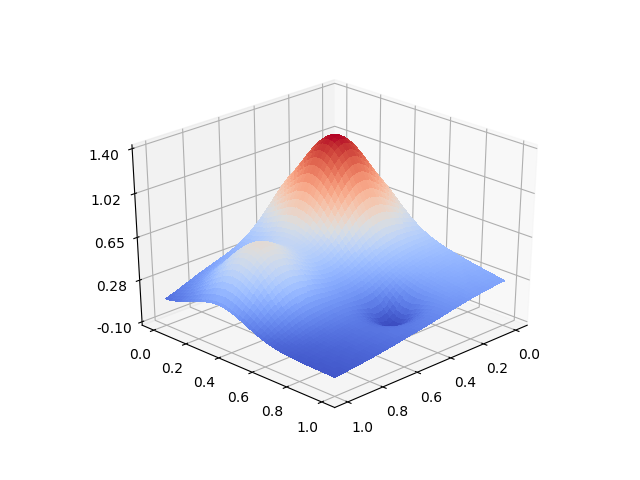
\includegraphics[width=\linewidth]{franke.png}
\captionof{figure}{The Franke test function plotted for $0\le x,y\le 1$. \label{fig:1}}
\end{Figure}



\section{Results and discussion}
\lipsum[3]

\section{Conclusion}
\lipsum[3]
\end{multicols}


\printbibliography[heading=bibintoc]
\end{document}



